\section{Công cụ dự báo cho một cell}\label{sec:congcu}

Công cụ dòng lệnh của đồ án gói PINN-semi, HiPINN và HiGBDT-V để dùng cho một cell bất kỳ, chỉ cần tệp đặc trưng sạc của cell đó. Lệnh thứ nhất học PINN-semi ở 30\,\% nhãn cho một bộ dữ liệu, lệnh thứ hai ước lượng SOH ở từng chu kỳ, lệnh thứ ba dự báo SOH, dung lượng và RUL từ một chu kỳ bất kỳ bằng HiPINN (\Cref{sec:e33pp}). Lần đầu dự báo cho một bộ, HiPINN được học trên các cell có nhãn của cùng fold với PINN-semi của công cụ, chọn cấu hình từng nhánh trên cell validation rồi lưu lại; cell được dự báo không tham gia khi học. Lịch sử SOH tới gốc là dung lượng đo của chính cell; cell chưa được đo dung lượng thì công cụ chỉ ước lượng SOH hiện tại (lệnh thứ hai), không dự báo. Lệnh thứ tư cập nhật SOH khi cell được đo dung lượng ở vài chu kỳ: ở mỗi chu kỳ không đo, HiGBDT-V (\Cref{sec:anchor}) ước lượng SOH từ lần đo gần nhất trước nó và đặc trưng sạc. Với cell 2C\_battery-8 của XJTU đo 11 lần trên 385 chu kỳ theo lịch mỗi $0{,}1L$, MAE ở các chu kỳ không đo là 2{,}1 ($\times10^{-3}$), so với 8{,}7 khi giữ nguyên lần đo gần nhất.

Lệnh thứ năm áp dụng HiPINN cho cả bốn bộ: với mỗi bộ, lấy cell test có số chu kỳ ở trung vị và dự báo từ 40\,\% số chu kỳ của nó (\Cref{fig:demo4}). MAE trên phần đời còn lại là 23{,}3 ở XJTU (cell 2C\_battery-1), 6{,}9 ở TJU (cell CY25-025\_1-\#4), 10{,}8 ở MIT (cell 2017-05-12\_battery-43) và 3{,}8 ở HUST (cell 7-1) ($\times10^{-3}$); ở TJU và HUST, HiPINN không kém nhánh tốt nhất của chính cell đó; ở XJTU, nhánh tốt nhất là HiGBDT (16{,}9); ở MIT, nhánh tốt nhất là nhánh theo đời (9{,}6). Mô hình của công cụ học trên 30\,\% cell có nhãn, ít hơn mức mọi cell train ở \Cref{sec:e33res}, và mỗi bộ chỉ có một cell, nên đây là minh hoạ chứ không phải số đánh giá.

\begin{figure}[!htbp]\centering
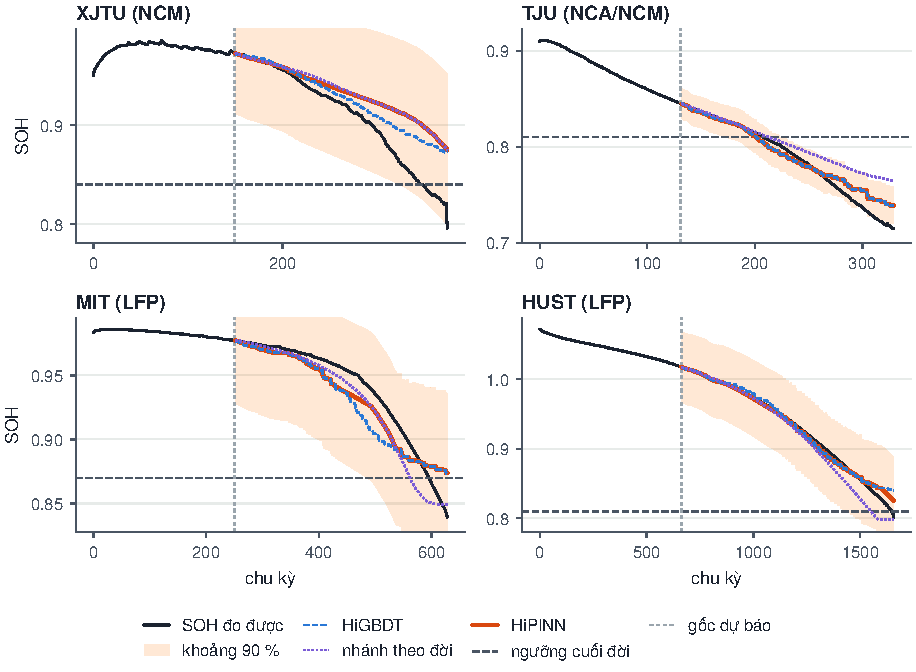
\includegraphics[width=\textwidth]{graphics/fig_demo_hipinn.pdf}
\caption[HiPINN cho một cell test của mỗi bộ dữ liệu]{HiPINN áp dụng cho bốn bộ dữ liệu qua công cụ dòng lệnh: với mỗi bộ, cell test có số chu kỳ ở trung vị, dự báo từ 40\,\% số chu kỳ của cell, lịch sử là dung lượng đo; mô hình học trên 30\,\% cell có nhãn của fold dùng cho công cụ. PINN-dự báo, nhánh thứ ba của HiPINN, không vẽ để hình dễ đọc.}\label{fig:demo4}
\end{figure}
